%%%%%%%%%%%%%%%%%%%
%%% 2025-02-04 %%%%
%%%%%%%%%%%%%%%%%%%
\section{Encuadre (2025-02-04)}
\begin{frame}\frametitle{Presentación del curso}
  \textbf{Objetivos:}
  \begin{itemize}
  \item Aprender los conceptos básicos para operar un robot móvil autónomo
  \item Implementar dichos conceptos en un ambiente simulado
  \item Familiarizar al estudiante con la plataforma ROS
  \end{itemize}
\end{frame}

\begin{frame}\frametitle{Ubicación en el plan de estudios}
  Bloque de ingeniería aplicada:
  \begin{figure}
    \centering
    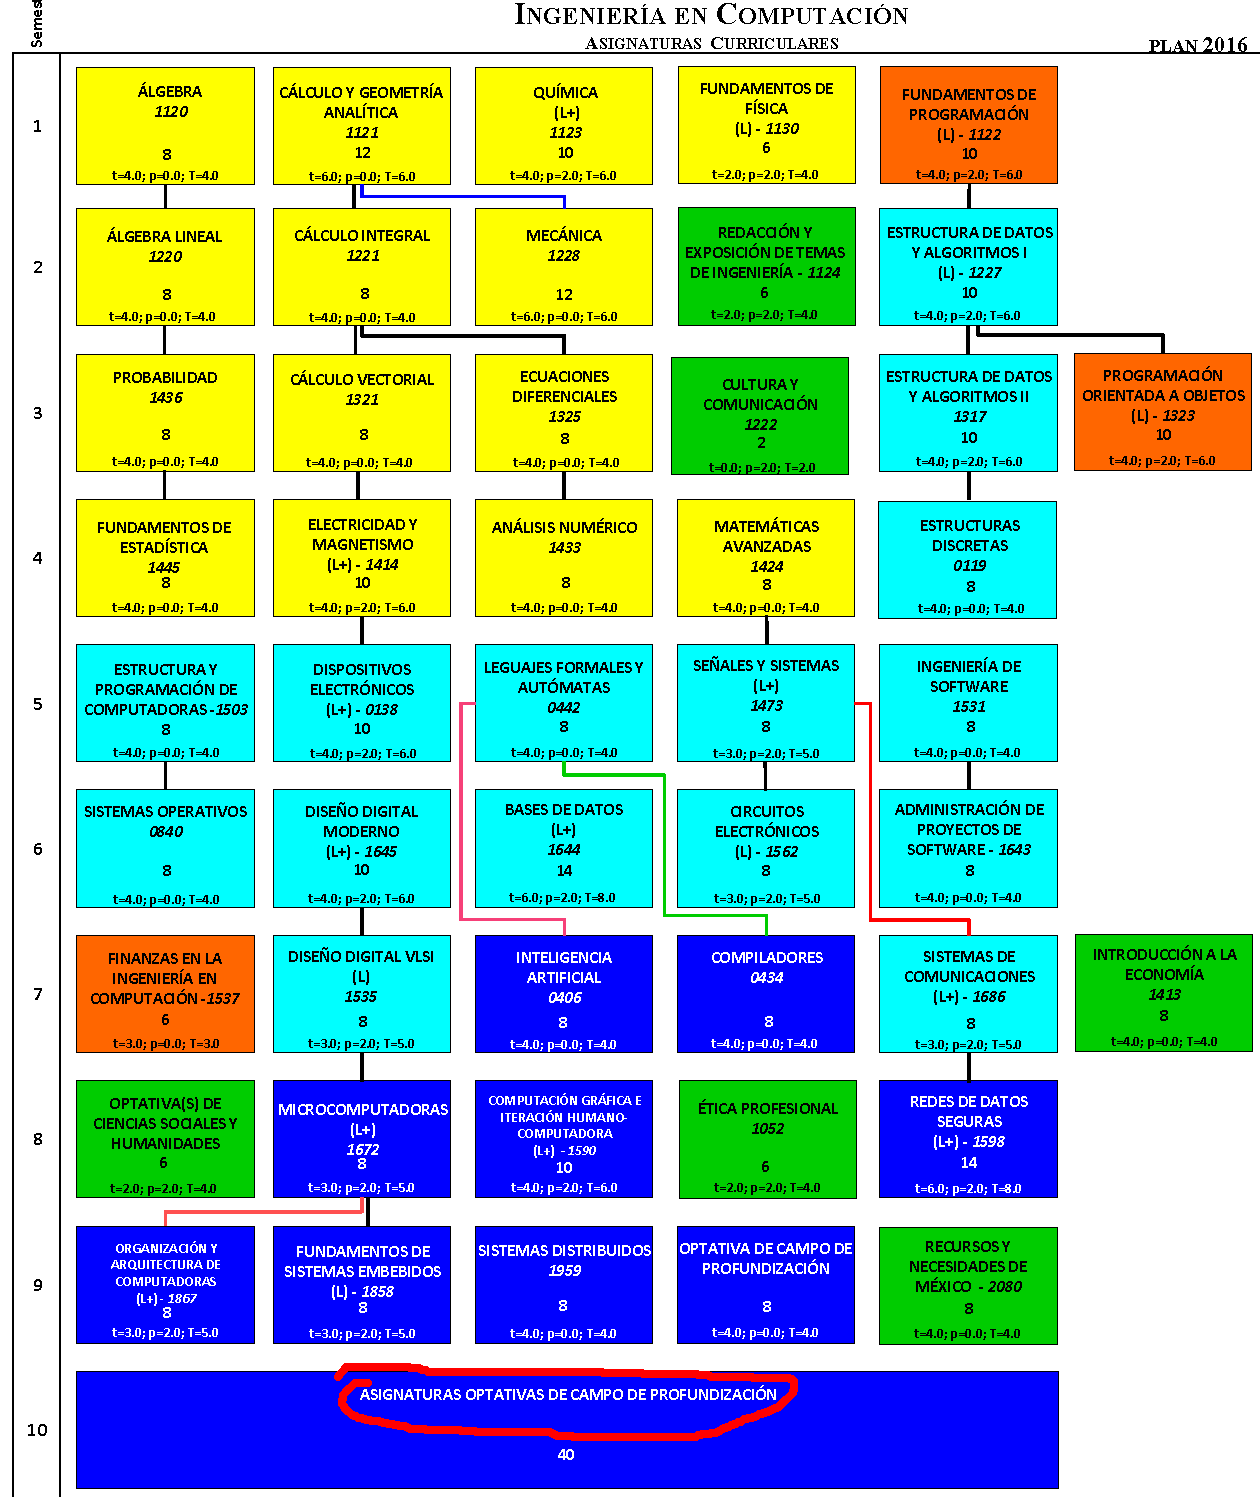
\includegraphics[width=0.3\textwidth]{Figures/Introduction/PlanComputacion.png}
    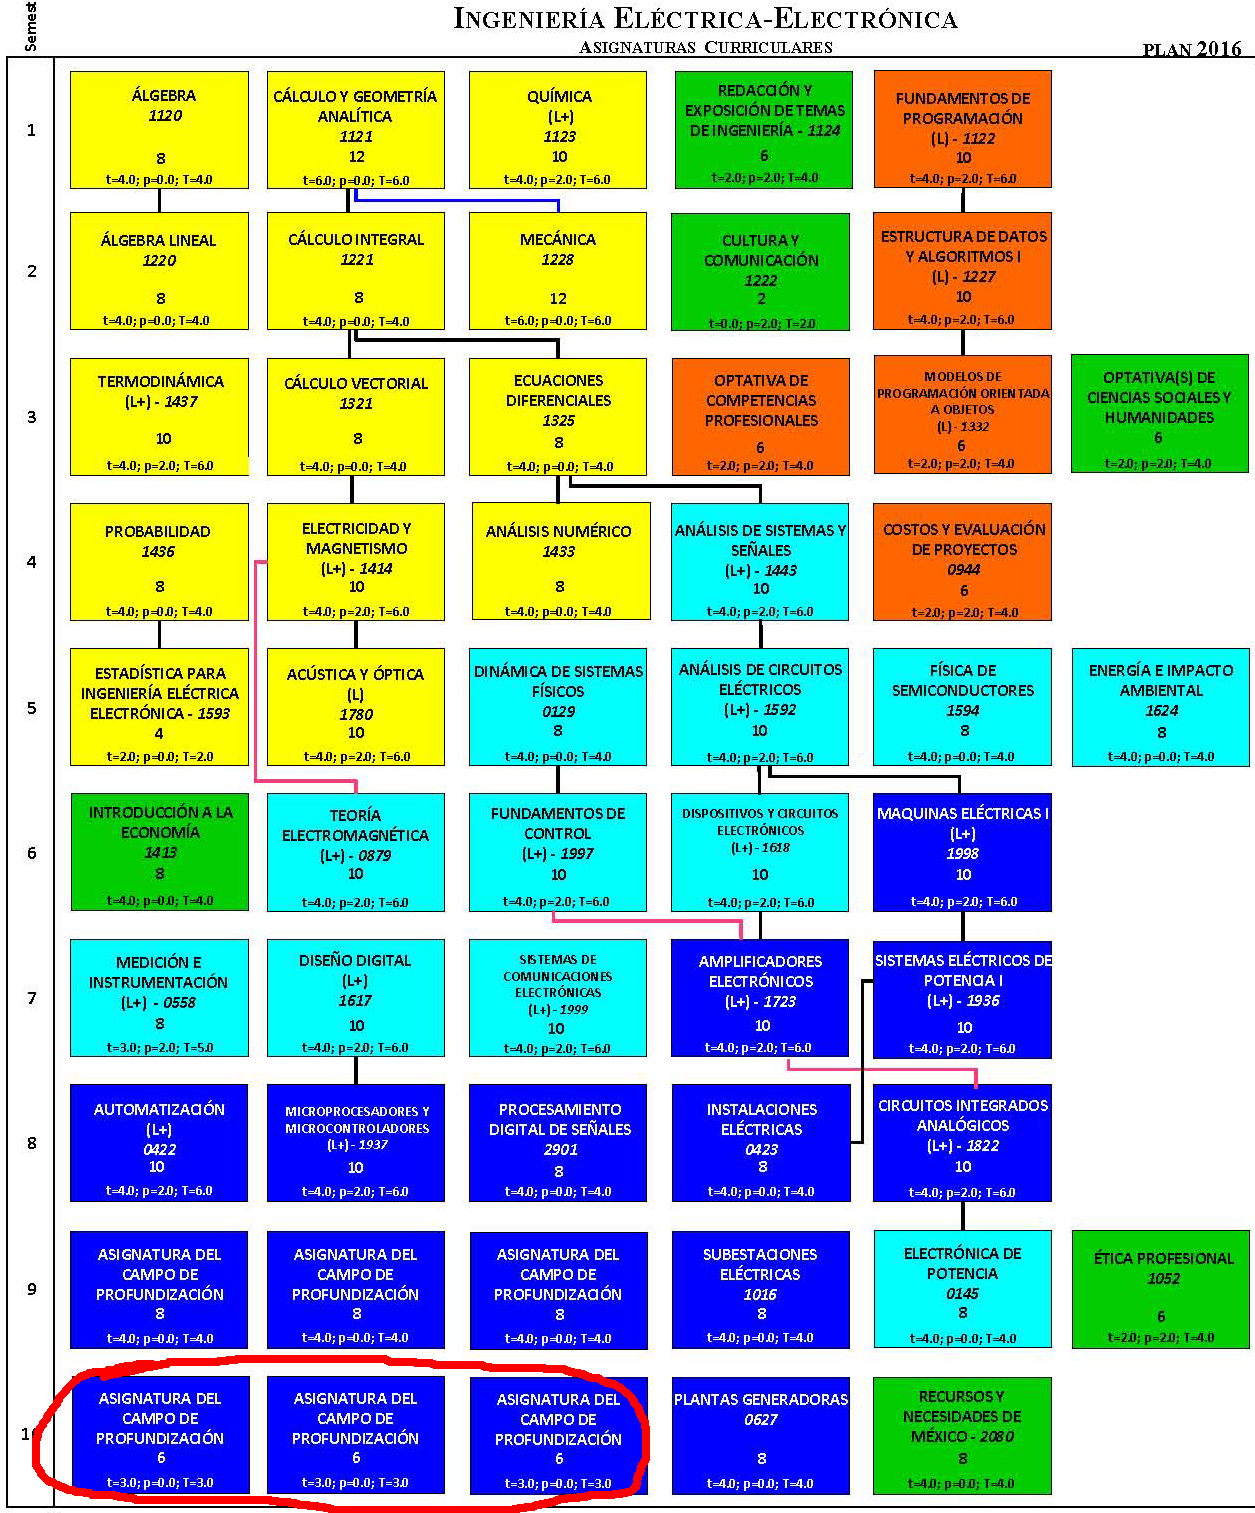
\includegraphics[width=0.3\textwidth]{Figures/Introduction/PlanElectronica.png}
    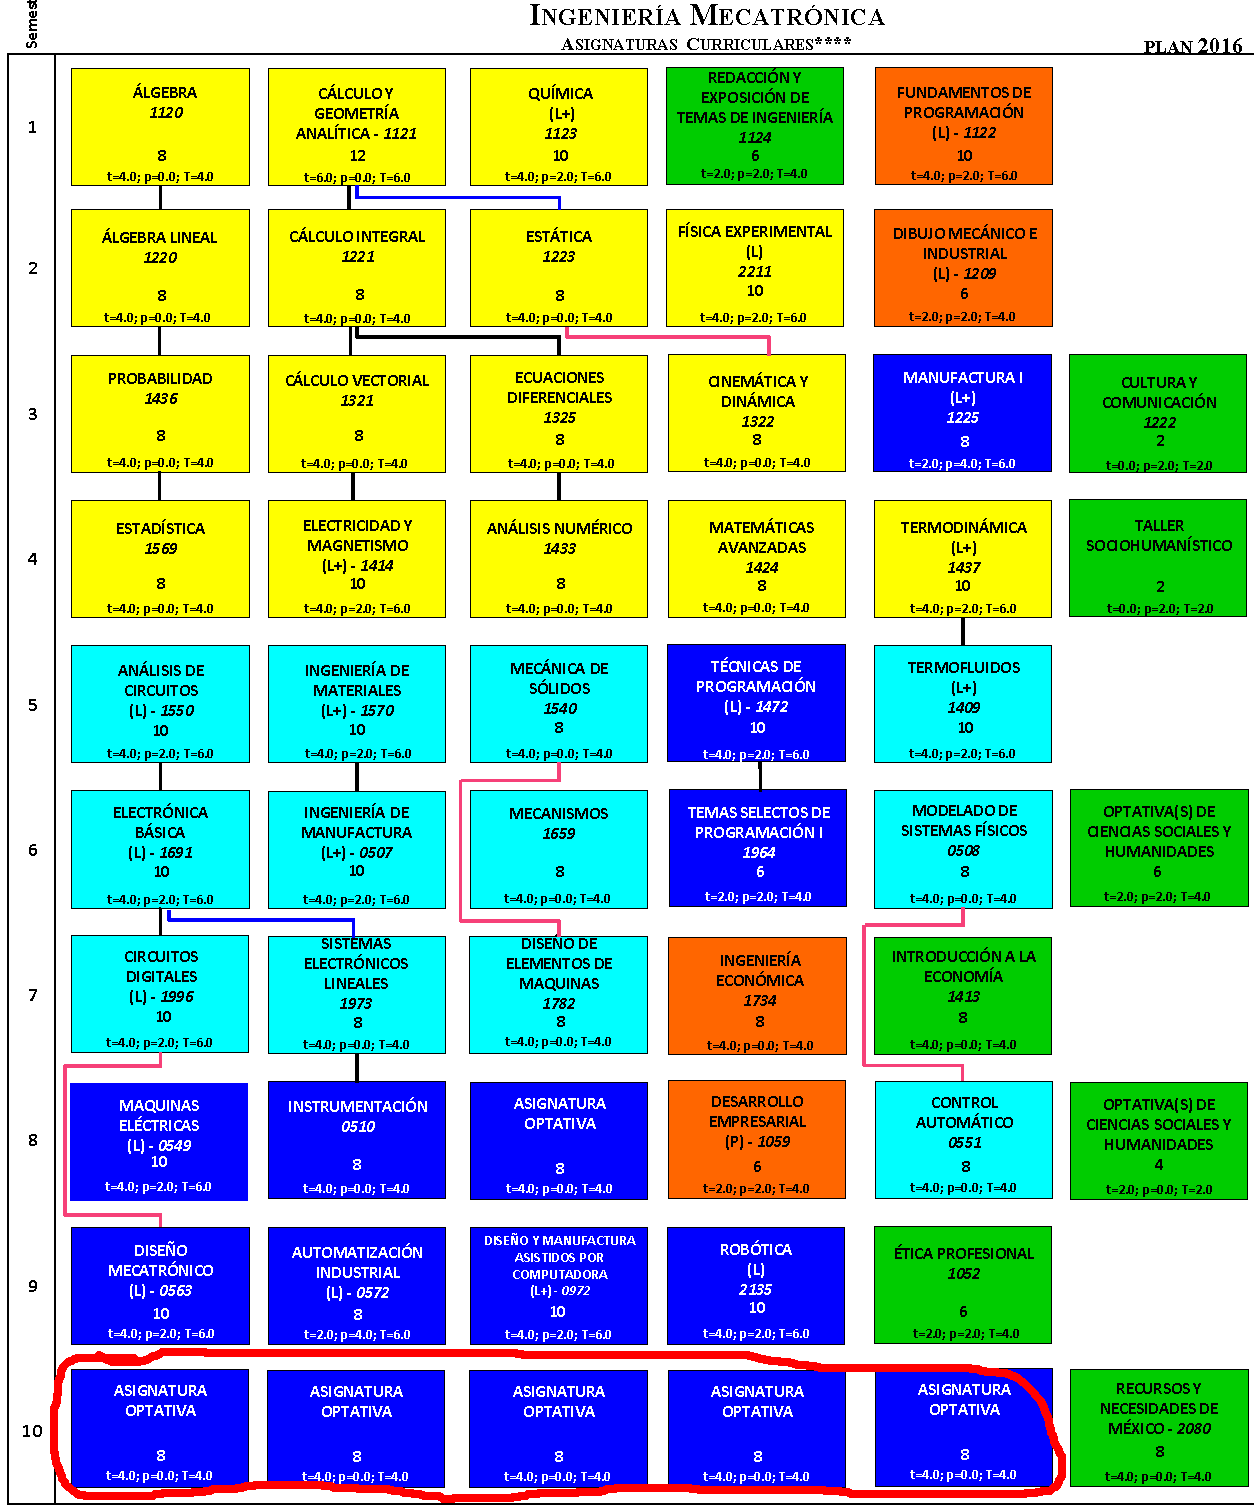
\includegraphics[width=0.3\textwidth]{Figures/Introduction/PlanMecatronica.png}
  \end{figure}
  El curso integra diversos conceptos vistos a lo largo de la carrera: cálculo, álgebra, geometría, probabilidad, estructuras de datos, control, entre otras. 
\end{frame}

\begin{frame}\frametitle{Contenido}
  \begin{enumerate}
  \item Introducción
    \begin{itemize}
    \item Componentes básicos de un robot móvil
    \item Herramientas de software para el desarrollo de robots móviles
    \end{itemize}
  \item Planeación de movimientos
    \begin{itemize}
    \item El problema de la planeación de movimientos
    \item Mapas geométricos y topológicos
    \item Descomposición en celdas, celdas de ocupación y diagramas de Voronoi
    \item Planeación de rutas mediante búsqueda en grafos
    \item Modelos cinemáticos: diferencial, omnidireccional, Ackermann
    \item Control de posición y seguimiento de trayectorias
    \end{itemize}
  \item Modelos reactivos
    \begin{itemize}
    \item Máquinas de estados finitas
    \item Campos potenciales artificiales
    \item Navegación mediante redes neuronales
    \item Navegación mediante algoritmos genéticos
    \end{itemize}
  \end{enumerate}
\end{frame}

\begin{frame}\frametitle{Contenido}
  \begin{enumerate}
    \setcounter{enumi}{3}
  \item Mapeo y localización
    \begin{itemize}
    \item Localización mediante filtro de Kalman extendido
    \item Localización mediante filtros de partículas
    \item Localización mediante Modelos Ocultos de Markov
    \item Creación de mapas mediante agrupamiento
    \item Localización y mapeo simultáneos
    \end{itemize}
  \item Conceptos básicos de visión artificial
    \begin{itemize}
    \item Imágenes y espacios de color
    \item Operadores morfológicos
    \item Extracción de características geométricas
    \item Visión 3D mediante imágenes RGB-D
    \item Redes neuronales artificiales
    \end{itemize}
  \item Conceptos básicos de manipulación
    \begin{itemize}
    \item Movimiento de cuerpo rígido
    \item Cinemáticas directa e inversa
    \item Planeación de trayectorias
    \item Seguimiento de trayectorias
    \end{itemize}
  \end{enumerate}
\end{frame}

\begin{frame}\frametitle{Contenido}
  \begin{enumerate}
    \setcounter{enumi}{6}
  \item Planeación de acciones
    \begin{itemize}
    \item Sistemas basados en reglas
    \item Procesos de Decisión de Markov
    \end{itemize}
  \item Herramientas para la interacción humano-robot
    \begin{itemize}
%    \item El modelo fuente-filtro para síntesis de voz
    \item Síntesis de voz con la biblioteca Festival
    \item Reconocimiento de palabras aisladas
    \item Reconocimiento de voz con la biblioteca CMU Sphinx
    \end{itemize}
  \end{enumerate}
  \textbf{Bibliografía recomendada:}
  \begin{itemize}
    \item \url{https://drive.google.com/drive/folders/1gb7VQJG5eUkCvCginRHHGn5lez6VASBJ?usp=sharing}
    \item \url{https://drive.google.com/drive/folders/1Epl2b51xEJzCvzfugBD1i7xGdKYdJucy?usp=sharing}
  \end{itemize}
  
\end{frame}

\begin{frame}\frametitle{Forma de trabajo}
  \begin{itemize}
  \item Horario: martes y jueves de 15:00 a 16:30.\\
  \item Para la realización de ciertas actividades se utilizará el simulador Gazebo junto con la plataforma ROS Noetic. Este software corre en el sistema operativo Ubuntu 20.04.4. Varias actividades implicarán escribir código para lo cual se utilizará el repositorio\\
    \url{https://github.com/mnegretev/Mobile-Robots-2025-2}\\
    Si no se desea instalar el sistema operativo de forma nativa, en el repositorio hay una máquina virtual con todo el software ya instalado.
  \item Para el uso del material del curso, se recomienda manejar las siguientes herramientas:
    \begin{itemize}
    \item Sistema operativo Ubuntu
    \item Lenguajes Python y C++
    \item Software de control de versiones Git
    \end{itemize}
    Un conocimiento a nivel introductorio es suficiente. En caso de no conocer las herramientas mencionadas, se recomienda buscar cursos gratuitos en \texttt{www.udacity.com} y \texttt{www.edx.org}
  \item La actividad integradora, las actividades de formación profesional y algunas secuencias unitarias incluyen la escritura de código. El alumno deberá completar el código utilizando las plantillas que ya se encuentran en el repositorio en línea en \url{https://github.com/mnegretev/Mobile-Robots-2025-2}
  \end{itemize}
\end{frame}

\begin{frame}\frametitle{Forma de trabajo}
  \begin{itemize}
  \item Se creará una rama del repositorio para cada estudiante donde podrá subir códigos. Para ello el estudiante debe tener cuenta en GitHub (gratuita) y se le darán permisos de escritura en el repositorio.
  \item Las instrucciones para cada entregable (secuencias unitarias, actividades de formación profesional, actividad integradora y la prueba objetiva) así como las fechas de entrega se publicarán en el aula virtual en Classroom:\\
    \[\]
    \Large{kjegylv}
    \normalsize{\\}
    \[\]
  \item Algunas actividades serán individuales y otras en equipo. En el Classroom se indicará la modalidad para cada actividad. 
  \item Las secuencias unitarias que impliquen la escritura de código, se subirán al repositorio en la rama asignada para cada estudiante.
  \item Las secuencias unitatias que no impliquen código se entregarán en papel al inicio de la clase en la fecha indicada.
  \end{itemize}
\end{frame}

\begin{frame}\frametitle{Forma de evaluar}
  Rubros a evaluar:
  \begin{table}
    \textbf{
  \begin{tabular}{lr}
    Actividades de formación profesional & 40\%\\
    Prueba objetiva    & 30\%\\
    Secuencias unitarias    & 25\%\\
    Actividad integradora  & 15\%
  \end{tabular}}
  \end{table}
  El examen final se exenta con 6.0. Si un alumno con calificación aprobatoria presenta el examen final, se entiende que renuncia a su calificación y el examen final contará el 100\%.
\end{frame}

\begin{frame}\frametitle
  \Large{\textbf{Todo comportamiento antiético causará una calificación de 0 en el entregable correspondiente o 5 en el curso, dependiendo de la falta.}}
  \normalsize
  \[\]
  Ejemplos:
  \begin{itemize}
  \item Copiar y pegar texto de internet
  \item Copiar el trabajo de otros compañeros
  \item Generar los trabajos empleando herramientas de IA
  \item Falsificar datos
  \item Falsificar referencias
  \end{itemize}
  En caso de sospecha de alguna falta, el alumno deberá defender su trabajo mediante una réplica oral. 
\end{frame}

\begin{frame}\frametitle{Forma de evaluar}
  \begin{itemize}
  \item Las secuencias unitarias se entregarán en papel al inicio de la clase en la fecha de entrega asignada. Si la secuencia incluye la escritura de código, éste deberá subirse al repositorio en la rama correspondiente. 
  \item Las prácticas consistirán en la escritura de código, que se subirá al repositorio en la rama correspondiente, y en la elaboración de un reporte escrito, que también se entregará impreso al inicio de la clase en la fecha asignada. 
  \item La actividad integradora final consistirá en la integración de los conceptos vistos en el curso para resolver una tarea simple relacionada con robots de servicio doméstico, por lo que también consistirá en la escritura de código y en un reporte escrito.
  \item Para las diversas actividades de evaluación se publicará en el Classroom el instrumento de evaluación correspondiente. Para el caso de prácticas y proyectos, se utilizará una rúbrica y para el caso de tareas, una lista de cotejo. 
  \end{itemize}
\end{frame}

\begin{frame}\frametitle{Evaluación de reportes de prácticas y proyecto}
  \begin{itemize}
  \item Los reportes de actividades de formación profesional y de la actividad integradora deberán contener al menos los siguientes puntos:
    \begin{itemize}
    \item Introducción (que incluya contexto, motivación, planteamiento del problema y objetivos)
    \item Marco teórico (donde se expliquen los conceptos utilizados en la práctica o proyecto)
    \item Desarrollo (donde se expliquen la implementación y las pruebas realizadas)
    \item Resultados (donde se reporten las diferentes pruebas de funcionamiento)
    \item Conclusiones (donde se discutan los resultados obtenidos y se plantee un trabajo futuro)
    \item Referencias
    \end{itemize}
  \item No hay extensión mínima ni máxima.
  \item No es necesario que los reportes sean extensos. Se prefiere que sean concisos.
  \item Las referencias deben ser sólo \textbf{publicaciones arbitradas} (libros, artículos de revista, memorias de congresos, entre otros). Se recomienda usar el buscador de la Dirección General de Bibliotecas de la UNAM (\url{https://www.dgb.unam.mx/})
  \item No es necesario incluir código en el reporte, para eso está el repositorio en línea.
  \item No es necesario reproducir las instrucciones de ejecución de cada práctica en el reporte.
  \item Las conclusiones deben estar basadas en los resultados presentados en el reporte. Las opiniones personales \textbf{NO} son conclusiones.
  \end{itemize}
\end{frame}

\begin{frame}\frametitle{Condición para continuar el curso}
  Se deberá enviar un correo electrónico a la dirección \texttt{marco.negrete@ingenieria.unam.edu} donde se indique lo siguiente:
  \begin{itemize}
  \item Manifestar que se conocen los siguientes puntos:
    \begin{itemize}
    \item Los objetivos del curso
    \item Los criterios de evaluación
    \item La forma de trabajo y la bibliografía recomendada
    \item Sanciones en caso de conductas antiéticas
    \end{itemize}
  \item Manifestar la aceptación de todos los puntos anteriores
  \end{itemize}
\end{frame}

